\section{Clustering}

\subsection{Methods}
\todo[inline]{Describe each clustering method with important parameters that could influence the outcome}
\subsubsection{K-Means} \label{theory:kmeans}
\todo[inline]{Explain the working of the algorithm}.
The most important parameter of the K-Means algorithm is the value of $k$.
This value determines the number of clusters to consider and has a big influence on the results \cite{ahmed_k-means_2020}.
One of the oldest methods to do this is to use an "elbow" plot \cite{kodinariya_review_2013}.
This method can be used to determine the best $k$ by applying the algorithm multiple times and estimateing the best $k$.
\begin{figure}[H]
  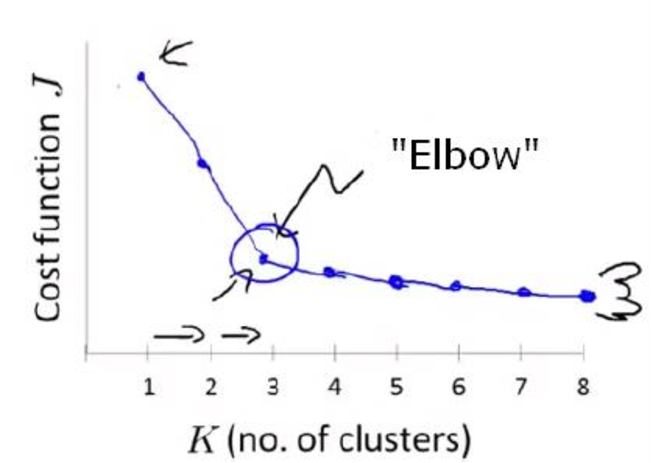
\includegraphics{TheorethicalFramework/dentification-of-Elbow-point.png}
  \caption{Illustration of determining $k$ using the "elbow" method \cite{kodinariya_review_2013}}
\end{figure}
However, sometimes the "elbow" is hard to find

\subsubsection{Affinity Propagation}:
\todo[inline]{Explain the working of the algorithm}.
\todo[inline]{Explain most important parameters}
\subsubsection{DBSCAN}:
\todo[inline]{Explain the working of the algorithm}.
\todo[inline]{Explain most important parameters}

\subsection{Evaluation methods} \label{theory:evaluate}
Clustering comparison measures are important in cluster analysis for external validation by comparing clustering solutions to a "ground truth" clustering \citep{vinh_information_nodate-2}.
These external validity indices are a common way to assess the quality of unsupervised machine learning methods like clustering \citep{warrens_understanding_2022}.
A method that could be used for this is the Rand Index \citep{rand_objective_1971}.
It is a commonly applied method for comparing two different cluster algorithms \citep{wagner_comparing_nodate}.
An improvement of this method is adjusted for chance by considering the similarity of pairwise cluster comparisons \citep{vinh_information_nodate-2}.
Both the Rand Index (RI) and Adjusted Rand Index (ARI) \citep{hubert_comparing_1985-1} report a value between 0 and 1.
Where 0 is for no-similarity and 1 for identical clusters.
Alternatives for RI are the Fowles-Mallows Index and Mirkin Metric.
However, these two methods have their disadvantages. Respectively, being sensitive to a few clusters and cluster sizes \citep{wagner_comparing_nodate}.
The ARI metric suffers from cluster size imbalance as well, so it only provides not a lot of information on smaller clusters \citep{warrens_understanding_2022}.
Instead, they recommend using the cluster index metric that was proposed by Fränti et al. \citep{franti_centroid_2014}.

Another popular group of methods is the information theoric-based measures \citep{vinh_information_nodate-2}.
This metric measures the information between centroids; the higher the value, the better \citep{vinh_information_nodate-2}.
\gls{mi} is such metric, which calculates the probability of an element belonging to cluster $C$ or $C`$.
But, is not easy to interpret as it does not have a maximum value \citep{wagner_comparing_nodate}.
To this end, \gls{nmi} can be used to report a value between 0 and 1 using the geometric mean \citep{strehl_cluster_2002}.
The metric exists also in an adjusted version as \gls{ami}.
This works in the same way as for the \gls{ari} and is mostly needed if the number of data items is small in comparison to the number of clusters \citep{vinh_information_nodate-2}. \newline

Besides the external validity measurements for clustering, it is also possible to use internal validation methods.
These metrics focus entirely on the intrinsic dataset properties, instead of relying on an external baseline cluster algorithm \cite{craenendonck_using_nodate}.
Assessing two important concepts of clustering: compactness and separation \cite{hassani_using_2017}.
Both studies, consider three different metrics and measure both concepts at the same time \cite{hassani_using_2017}:
\begin{enumerate}
  \item \gls{chi} \citep{calinski_dendrite_1974-1} is used to measure the cluster variance (well-separated clusters) and low variance within the clusters (tightly coupled data). A high score indicates better clustering.
  \item Silhouette Index \citep{rousseeuw_silhouettes_1987} this metric is similar, by also measuring cohesion within clusters and separation of clusters. However, this metric uses the pairwise distance \cite{hassani_using_2017}. A score of -1 indicates incorrect clustering and +1 for dense clusters \cite{rousseeuw_silhouettes_1987}.
  \item Davies-Bouldin \citep{davies_cluster_1979} uses the average distance between centroids. A lower score indicates good clustering.
\end{enumerate}

K-Means scores relatively high for \gls{chi} \citep{craenendonck_using_nodate,hassani_using_2017} and SI \citep{craenendonck_using_nodate}.
The same applies to DBSCAN, which scores relatively high on SI and DB due to the sensitivity of noise \cite{craenendonck_using_nodate}.
% Thus, these metrics are difficult to use for very different cluster algorithms \cite{craenendonck_using_nodate}.
\subsubsection{Existing literature}
%A recent and much-cited study uses \gls{ari} and accuracy as metrics for evaluating K-Means \cite{ahmed_k-means_2020}.
%The accuracy is measured by calculating the percentage of the correct predicted labels and their truth labels.
Comparable studies with differential privacy use external validation \citep{xia_distributed_2020-1, sun_privbv_2022}.
Their experiment setup uses a so-called non-private cluster algorithm as external validation.
This cluster algorithm is trained without the perturbed data and compared with the same clustering algorithm that is trained with perturbed data.
Thus, the non-private variant functions as an external validation by providing the ground truth.

They compare the mutual information between a baseline cluster algorithm using \gls{ami} \citep{9679364} or \gls{nmi} \citep{xia_distributed_2020-1,sun_privbv_2022}.
Another study for evaluating \gls{dp} with \gls{ap} uses both \gls{ari} and \gls{ami}.
In addition to mutual information and rand index scores, it is also not uncommon to calculate the error between the two cluster algorithm's centroids \citep{xia_distributed_2020-1, 9679364}.
These two studies used Relative Error (RE) for this.